\documentclass[10pt,aspectratio=169]{beamer}
%\setbeameroption{show notes on second screen=right}

\usetheme{Madrid}


\usetheme[progressbar=frametitle]{metropolis}
\usecolortheme{rose} %beaver, dolphin, crane, 


\setbeamersize{text margin left=4mm, text margin right=4mm}


\usecolortheme{default}
\setbeamertemplate{navigation symbols}{}
\setbeamertemplate{footline}[frame number]
\usepackage[utf8]{inputenc}
\usepackage[T1]{fontenc}

\usepackage{amsmath, amssymb, bm}
\usepackage{booktabs}
\usepackage{graphicx}
\usepackage{ragged2e}
\usepackage{hyperref}
\hypersetup{colorlinks=true, urlcolor=blue}

\title[Competing under Information Heterogeneity]{Competing under Information Heterogeneity:\\ Evidence from Auto Insurance}
\author[Cosconati, Fan, Jin, Wu]{Marco Cosconati \and Yi Xin Fan \and Yizhou Jin \and Wu}
\institute{IVASS, Bank of Italy \and Caltech \and Caltech \and University of Toronto}
\date{July 8, 2025}

\begin{document}

% 1
\begin{frame}
  \titlepage
\end{frame}

% 2
\begin{frame}{Motivation}
\justifying
\begin{itemize}
  \item Firms increasingly differ in \emph{information precision} (data access/analytics) and in \emph{cost structures}.
  \item This creates information asymmetries \emph{between} firms (beyond classic buyer--seller asymmetry).
  \item Policy interest: regulations that equalize or share consumer risk information (e.g., centralized ``risk bureau'').
\end{itemize}
\end{frame}

% 3
\begin{frame}{Research Questions}
\justifying
\begin{itemize}
  \item How does heterogeneous information across insurers shape pricing, sorting, and market power?
  \item What happens to prices, surplus, profits, and sorting if information is shared/standardized?
  \item Distributional effects: who gains (low vs. high risk)? Efficiency effects: matching and costs?
\end{itemize}
\end{frame}

% 4
\begin{frame}{Contributions}
\justifying
\begin{itemize}
  \item A tractable model of imperfect competition with firm-specific information precision and costs.
  \item New identification/estimation strategy using offered-price distributions and demand to recover signals.
  \item Evidence from Italian auto liability insurance with rich panel linking consumers across insurers.
  \item Counterfactuals: centralized risk bureau, full information, and privacy/high-variance restrictions.
\end{itemize}
\end{frame}

% 5
\begin{frame}{Institutional Background: Italian Auto Liability (RCA)}
\justifying
\begin{itemize}
  \item Mandatory, annual, exclusive contracts; insurers cannot reject consumers.
  \item Large market: $\approx$31M contracts in 2018; $\approx$50 national competitors.
  \item Key contract features widely standardized; little use of deductibles.
\end{itemize}
\end{frame}

% 6
\begin{frame}{Data: IVASS IPER Microdata}
\justifying
\begin{itemize}
  \item Nationally representative matched insurer--insuree panel with claims frequency/severity, premiums, coverage.
  \item Tracks policyholders across insurers and time $\Rightarrow$ measure risk using ex-post claims panel.
  \item Focus sample: new customers in Rome (2013--2021); top 10 firms + fringe group.
\end{itemize}
\end{frame}

%%%%%%%%%%%%%%%%%%%%%%%%%%%%%%%%%%%%%%%%%%%%%%%%%%%
\section{Descriptive evidence}

% 7
\begin{frame}{Sample \& Summary Statistics}
\justifying
\begin{itemize}
  \item $N \approx 124{,}428$ contracts; avg premium $\approx \,€478$; within-year claim rate $\approx 0.08$.
  \item Demographics/vehicle: 56\% male; avg age 48; BM class $\approx 2$; car age $\approx 8.3$ years.
\end{itemize}
\begin{figure}[H]
%\caption{}
\centering{}%
\begin{tabular}{cc}
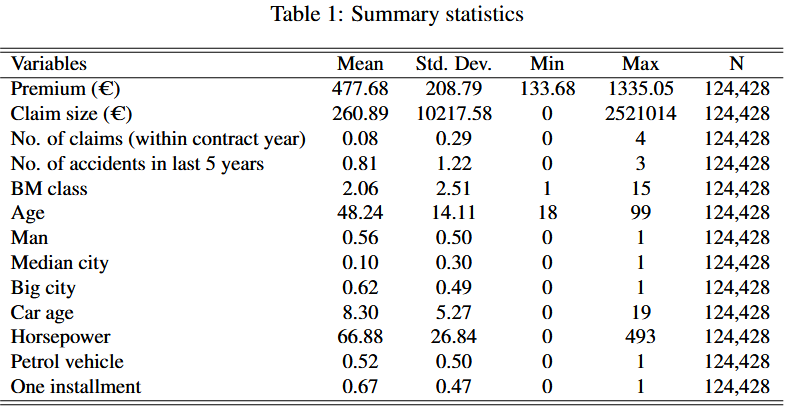
\includegraphics[scale=0.41]{Figures/Tab1.png}
\end{tabular}
\end{figure}
\end{frame}

% 8
\begin{frame}{Stylized Facts: Price Variation \& Sorting}
\begin{figure}[H]
%\caption{}
\centering{}%
\begin{tabular}{cc}
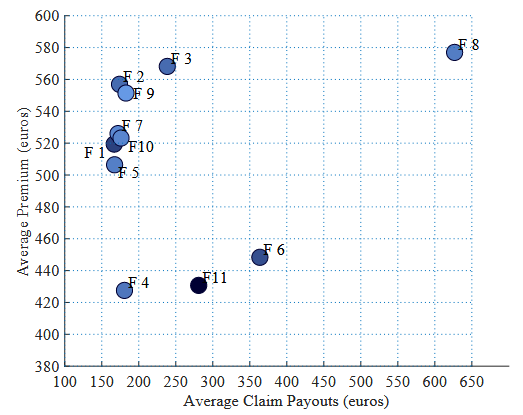
\includegraphics[scale=0.47]{Figures/Fig1.png}
\end{tabular}
\end{figure}
\vspace{0.75em}
\begin{itemize}
  \item Large cross-firm variation in average premiums even at similar average risks/market shares.
  \item Firms with higher average claim costs attract riskier consumers $\Rightarrow$ sorting across firms.
\end{itemize}
\end{frame}

% =========================
% INSERT THIS BEFORE SLIDE 9
% =========================
\begin{frame}{How we built Figure 2 (Savings distribution)}
\small
\textbf{Goal.} Show the distribution of individuals' savings (in UF) for the analysis sample, with extreme values trimmed to improve readability.

\vspace{0.6em}
\textbf{Data.} Administrative SCOMP records. Savings come from the request file (\textit{Solicitudes}): the AFP-reported balance in UF at the time of request. We restrict to the paper’s analysis sample used elsewhere in the slides.

\vspace{0.6em}
\textbf{Sample used for the figure.}
\begin{itemize}\itemsep2pt
  \item Start from the accepted certificates used in the analysis (one row per \textit{certificado de saldo}).
  \item Keep annuity modality RV inmediata only; drop observations with ELD and with months guaranteed $\neq 0$ to match the core sample used in the paper.
  \item Merge in savings from \textit{Solicitudes} (balance in UF). If multiple requests exist for a certificate, keep the request closest (in time) to acceptance.
\end{itemize}

\vspace{0.6em}
\textbf{Cleaning and construction.}
\begin{itemize}\itemsep2pt
  \item Remove missing/implausible balances (nonpositive UF).
  \item Compute the 99th percentile of savings and \emph{truncate} the right tail at that value (values above p99 are set to p99) to avoid the plot being dominated by very large balances.
\end{itemize}

\vspace{0.6em}
\textbf{Plot.}
\begin{itemize}\itemsep2pt
  \item Histogram (or kernel density) of truncated savings in UF; x-axis capped at p99; y-axis as share of individuals.
  \item Label: “1 UF $\approx$ \$40 (intuition only).”
\end{itemize}

\vspace{0.6em}
\textbf{Reproducibility (sketch).}
\begin{itemize}\itemsep2pt
  \item Compute p99: $q_{0.99} = \mathrm{quantile}(\text{savings}, 0.99)$; set $\text{sav\_trunc}=\min(\text{savings}, q_{0.99})$.
  \item Plot histogram of \texttt{sav\_trunc} with fixed binning.
\end{itemize}

\vspace{0.6em}
\textbf{Interpretation.} Figure 2 summarizes the cross-section of resources available at purchase. Truncating at p99 preserves the shape of the bulk of the distribution and prevents outliers from compressing the x-axis.
\end{frame}


% 9 (NEW SLIDE - to be inserted before current slide 9)
\begin{frame}{Measuring Information Precision: Methodology}
\justifying
\textbf{How was Figure 2 created?}
\begin{enumerate}
\item \textbf{Step 1: Construct individual risk measures}
\begin{itemize}
\item Panel regression of claim counts with individual fixed effects
\item Log-normal regression of claim severity conditional on accident
\item Risk measure = Expected frequency × Expected severity
\end{itemize}
\item \textbf{Step 2: Firm-specific premium-risk regressions}
\begin{itemize}
\item For each firm $j$: $\text{Premium}_{ij} = \alpha_j + \beta_j \cdot \text{Risk}_i + \varepsilon_{ij}$
\item Higher $\beta_j$ suggests firm's prices are more responsive to actual risk
\end{itemize}
\item \textbf{Step 3: Bootstrap standard errors}
\begin{itemize}
\item 200 bootstrap replications accounting for generated regressor
\item Produces 95\% confidence intervals shown as error bars
\end{itemize}
\end{enumerate}
\vspace{0.5em}
\textbf{Key insight:} Variation in $\beta_j$ across firms indicates heterogeneous risk-rating precision
\end{frame}

% 9
\begin{frame}{Heterogeneity in Information Precision}
\justifying
\begin{itemize}
  \item \textcolor{red}{ADD WHY WE NEED A MODEL}
  \item Measure how strongly each firm’s premium responds to realized consumer risk (ex-post panel-based risk).
  \item Strong cross-firm differences in premium–risk slopes $\Rightarrow$ heterogeneous precision.
\end{itemize}|
\vspace{0.75em}
\begin{figure}[H]
%\caption{}
\centering{}%
\begin{tabular}{cc}
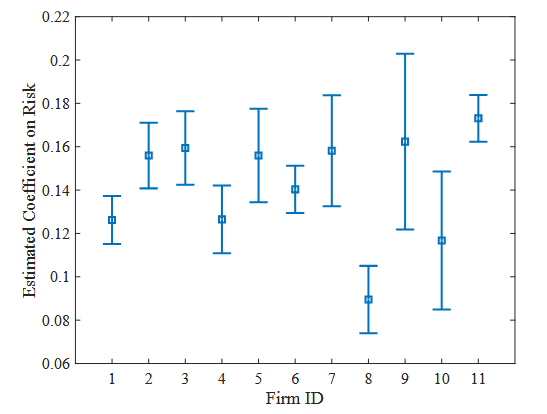
\includegraphics[scale=0.45]{Figures/Fig2.png}
\end{tabular}
\end{figure}
\end{frame}

%%%%%%%%%%%%%%%%%%%%%%%%%%%%%%%%%%%%%%%%%%%%%%%%%%%
\section{Model \& Estimation}

% 10
\begin{frame}{Conceptual Framework (Overview)}
\justifying
\begin{itemize}
  \item $J$ insurers; standardized product; no outside option.
  \item Consumer true risk $\theta$ (expected cost/year) unobserved ex ante.
  \item Firm $j$ observes a private signal $\hat{\theta}_j$ with precision that differs across firms.
\end{itemize}
\end{frame}

% 11
\begin{frame}{Signal Structure}
\justifying
\begin{equation}
\hat{\theta}_j \sim \mathcal{N}(\theta,\ \sigma_j^2), \quad \text{independent across } j \mid \theta, 
\label{eq:signal}
\end{equation}
\begin{itemize}
  \item Lower $\sigma_j^2$ $\Rightarrow$ higher information precision for firm $j$.
  \item Signals are used to form posterior beliefs about $\theta$ \emph{conditional on selection}.
\end{itemize}
\end{frame}

% 12
\begin{frame}{Risk Rating \& Pricing}
\justifying
\begin{equation}
p_j(\hat{\theta}_j) \;=\; \alpha_j \;+\; \beta_j \, \mathbb{E}[\theta \mid \hat{\theta}_j,\, D=j],
\label{eq:pricing}
\end{equation}
\begin{itemize}
  \item $\alpha_j$: baseline markup; $\beta_j$: pass-through/sensitivity to risk rating.
  \item $\mathbb{E}[\theta \mid \hat{\theta}_j, D=j]$ embeds selection $\Rightarrow$ nonlinearity in $\hat{\theta}_j$.
\end{itemize}
\end{frame}

% 13
\begin{frame}{Demand}
\justifying
\begin{itemize}
  \item Consumers choose one insurer; utility depends on price and observable characteristics.
  \item No outside option (mandatory purchase) $\Rightarrow$ shares across $J$ firms sum to 1.
  \item Preference parameters allowed to vary with observables and risk type.
\end{itemize}
\end{frame}

% 14
\begin{frame}{Identification: Intuition}
\justifying
\begin{itemize}
  \item Offered price is (strictly) increasing in the firm’s private signal (auction-style monotonicity).
  \item Use observed \emph{transaction} prices + demand model to invert to \emph{offered-price} distributions by firm.
  \item How average prices move with risk identifies $(\alpha_j,\beta_j)$; residual dispersion $\Rightarrow \sigma_j^2$.
\end{itemize}
\end{frame}

% 15
\begin{frame}{Estimation Steps}
\justifying
\begin{enumerate}
  \item Estimate demand and map transaction prices/shares to offered-price CDFs (firm-specific, nonparametric).
  \item Recover pricing coefficients $(\alpha_j,\beta_j)$ from price–risk relationships.
  \item Use price dispersion to identify signal variance $\sigma_j^2$ (information precision).
  \item Back out firm cost parameters from first-order conditions.
\end{enumerate}
\end{frame}

% 16
\begin{frame}{Data Construction of Risk (Two-Part Model)}
\justifying
\begin{itemize}
  \item Panel regressions to estimate individual risk:
  \begin{itemize}
    \item Frequency (accident counts with FE) and severity (conditional paid amount).
    \item Multiply predicted frequency $\times$ predicted severity $\Rightarrow$ expected cost per year.
  \end{itemize}
  \item Controls for contract features (coverage, restrictions, devices) mitigate moral-hazard confounds.
\end{itemize}
\end{frame}

% 17
\begin{frame}{Results: Firm Heterogeneity}
\justifying
\begin{itemize}
  \item Large differences across firms in information precision ($\sigma_j^2$), pricing sensitivity ($\beta_j$), and costs.
  \item Firms with less accurate risk-rating tend to have \emph{more efficient} claim-processing costs.
  \item Baseline sorting: higher-risk consumers concentrate at firms with higher average claim payouts.
\end{itemize}
\end{frame}

% 18
\begin{frame}{Results: Price Sensitivity \& Markups}
\justifying
\begin{itemize}
  \item Estimated $\beta_j$ varies markedly: some firms’ prices are much more responsive to risk.
  \item Baseline markups ($\alpha_j$) differ, consistent with market power from information advantages.
\end{itemize}
\vspace{0.75em}
\begin{center}
\textit{[Insert plot: distribution of $\beta_j$ and $\alpha_j$ across firms.]}
\end{center}
\end{frame}

% 19
\begin{frame}{Counterfactuals: Information Policies}
\justifying
\begin{itemize}
  \item \textbf{Centralized Risk Bureau}: aggregate firms’ signals (weighted by precision), share equally with all.
  \item \textbf{Full Information Benchmark}: firms observe true $\theta$ (eliminate information asymmetry).
  \item \textbf{Privacy/Restriction}: firms can only use basic information; set $\sigma_j^2$ to the worst observed.
\end{itemize}
\end{frame}

% 20
\begin{frame}{Counterfactual Results: Prices \& Welfare}
\justifying
\begin{itemize}
  \item Average premiums fall by $\sim$21.6\% (bureau) to $\sim$25.7\% (full information).
  \item Consumer surplus rises by $\sim$15.7\% (bureau), close to $\sim$16.9\% (full information).
  \item Firm profits decline on average; losses largest for firms with advanced risk-rating tech.
\end{itemize}
\vspace{0.75em}
\begin{center}
\textit{[Insert bar chart: $\Delta$ premium, $\Delta$ CS, $\Delta$ profit under each scenario.]}
\end{center}
\end{frame}

% 21
\begin{frame}{Distributional Effects by Risk Type}
\justifying
\begin{itemize}
  \item Bureau/full-info mainly benefit \emph{low-risk} consumers via sharper risk-based pricing.
  \item Privacy/high-variance benefits \emph{high-risk} consumers (harder to distinguish from low-risk).
\end{itemize}
\vspace{0.75em}
\begin{center}
\textit{[Insert plot: CS changes by risk decile under each scenario.]}
\end{center}
\end{frame}

% 22
\begin{frame}{Mechanism: Competition \& Undercutting}
\justifying
\begin{itemize}
  \item Equalizing information weakens incumbents’ info-based market power.
  \item Common risk evaluation $\Rightarrow$ more effective undercutting $\Rightarrow$ stronger price competition.
\end{itemize}
\end{frame}

% 23
\begin{frame}{Sorting \& Efficiency}
\justifying
\begin{itemize}
  \item With equal access to risk, firms more efficient at processing claims re-target higher-risk consumers.
  \item Sorting shifts from info advantages to cost specialization.
  \item Efficiency gains: avg cost $\downarrow$ by $\sim$3.7\% (full info) and by $\sim€12$ per contract (bureau).
\end{itemize}
\vspace{0.75em}
\begin{center}
\textit{[Insert figure: change in sorting patterns (risk $\times$ firm) vs. baseline.]}
\end{center}
\end{frame}

% 24
\begin{frame}{Robustness (Selected)}
\justifying
\begin{itemize}
  \item Alternative risk measures and controls for contract features.
  \item Bootstrapped uncertainty accounting for generated regressors.
  \item Poisson checks: premiums predicting claim counts; similar cross-firm heterogeneity.
\end{itemize}
\vspace{0.75em}
\begin{center}
\textit{[Insert table/figure: robustness summaries.]}
\end{center}
\end{frame}

% 25
\begin{frame}{Policy Implications}
\justifying
\begin{itemize}
  \item Centralized information can materially lower prices and raise consumer surplus.
  \item Distributional trade-offs: low-risk consumers gain more under information sharing; high-risk under privacy.
  \item Industry composition effects: advanced-screening firms lose profits; potential dynamic innovation effects.
\end{itemize}
\end{frame}

% 26
\begin{frame}{Limitations}
\justifying
\begin{itemize}
  \item Abstract from dynamic pricing/learning and multi-product cross-selling mechanisms.
  \item Treat signals as reduced-form precision differences (black box of algorithms/data).
  \item Focus on new customers (tenure $=0$) to avoid dynamics $\Rightarrow$ external validity caveats.
\end{itemize}
\end{frame}

% 27
\begin{frame}{Paths for Future Work}
\justifying
\begin{itemize}
  \item Dynamic extensions with learning and switching costs.
  \item Endogenous investment in information precision and costs (innovation incentives under policy).
  \item Generalization to other selection markets (credit, health, annuities) under heterogeneous information.
\end{itemize}
\end{frame}

% 28
\begin{frame}{Takeaways}
\justifying
\begin{itemize}
  \item Information heterogeneity shapes pricing power, sorting, and efficiency.
  \item Centralized sharing can compress prices and reorient sorting toward cost efficiency.
  \item Welfare gains are sizable, with clear distributional patterns across risk types.
\end{itemize}
\end{frame}

% 29
\begin{frame}{Appendix: Risk Construction Details}
\justifying
\begin{itemize}
  \item Frequency model with individual fixed effects; severity model (log amounts).
  \item Predicted risk = $\widehat{\text{freq}} \times \widehat{\text{severity}}$; controls for contract features.
\end{itemize}
\vspace{0.75em}
\begin{center}
\textit{[Insert table/figure: frequency \& severity regression summaries.]}
\end{center}
\end{frame}

% 30
\begin{frame}{Appendix: Identification Sketch}
\justifying
\begin{itemize}
  \item Monotonicity of offers in signals $\Rightarrow$ order-preserving mapping to signal quantiles.
  \item Demand-implied mapping from transactions to offers recovers firm-specific offer CDFs.
  \item Price--risk slope pins down $(\alpha_j,\beta_j)$; residual dispersion identifies $\sigma_j^2$.
\end{itemize}
\end{frame}

% 31
\begin{frame}{Q\&A}
\centering
\Large Questions?
\end{frame}

\end{document}
